\documentclass{article}
\usepackage{graphicx, tikz-cd, float, titlepic, booktabs} % Required for inserting images
\usepackage{pgfplots}
\pgfplotsset{compat=1.15}
\usepackage{mathrsfs}
\usetikzlibrary{arrows}
\usepackage{amsmath, amssymb, amsthm, amsfonts, siunitx, physics, gensymb}
\AtBeginDocument{\RenewCommandCopy\qty\SI}
\usepackage[version=4]{mhchem}
\usepackage[most,many,breakable]{tcolorbox}
\usepackage{xcolor, fancyhdr, varwidth}
\usepackage[Glenn]{fncychap}
%Options: Sonny, Lenny, Glenn, Conny, Rejne, Bjarne, Bjornstrup
\usepackage{hyperref, cleveref}
\usepackage{icomma, enumitem} %comma as decimal and continue enumerate with [resume]
\usepackage{plimsoll} %use standard state symbol with \stst
\usepackage[danish]{babel}
%%%%%%%%%%%%%%%%%%%%%%%%%%%%%%
% SELF MADE COLORS
%%%%%%%%%%%%%%%%%%%%%%%%%%%%%%
\definecolor{myg}{RGB}{56, 140, 70}
\definecolor{myb}{RGB}{45, 111, 177}
\definecolor{myr}{RGB}{199, 68, 64}
\definecolor{mytheorembg}{HTML}{F2F2F9}
\definecolor{mytheoremfr}{HTML}{00007B}
\definecolor{mylenmabg}{HTML}{FFFAF8}
\definecolor{mylenmafr}{HTML}{983b0f}
\definecolor{mypropbg}{HTML}{f2fbfc}
\definecolor{mypropfr}{HTML}{191971}
\definecolor{myexamplebg}{HTML}{F2FBF8}
\definecolor{myexamplefr}{HTML}{88D6D1}
\definecolor{myexampleti}{HTML}{2A7F7F}
\definecolor{mydefinitbg}{HTML}{E5E5FF}
\definecolor{mydefinitfr}{HTML}{3F3FA3}
\definecolor{notesgreen}{RGB}{0,162,0}
\definecolor{myp}{RGB}{197, 92, 212}
\definecolor{mygr}{HTML}{2C3338}
\definecolor{myred}{RGB}{127,0,0}
\definecolor{myyellow}{RGB}{169,121,69}
\definecolor{myexercisebg}{HTML}{F2FBF8}
\definecolor{myexercisefg}{HTML}{88D6D1}
%%%%%%%%%%%%%%%%%%%%%%%%%%%%%%%%%%%%%%%%%%%%%%%%%%%%%%%%%%%%%%%%%%%%%%
% Box environments for theorems and problems
%%%%%%%%%%%%%%%%%%%%%%%%%%%%%%%%%%%%%%%%%%%%%%%%%%%%%%%%%%%%%%%%%%%%%
\setlength{\parindent}{1cm}
%================================
% Question BOX
%================================
\makeatletter
\newtcbtheorem{question}{Opgave}{enhanced,
	breakable,
	colback=white,
	colframe=myb!80!black,
	attach boxed title to top left={yshift*=-\tcboxedtitleheight},
	fonttitle=\bfseries,
	title={#2},
	boxed title size=title,
	boxed title style={%
			sharp corners,
			rounded corners=northwest,
			colback=tcbcolframe,
			boxrule=0pt,
		},
	underlay boxed title={%
			\path[fill=tcbcolframe] (title.south west)--(title.south east)
			to[out=0, in=180] ([xshift=5mm]title.east)--
			(title.center-|frame.east)
			[rounded corners=\kvtcb@arc] |-
			(frame.north) -| cycle;
		},
	#1
}{def}
\makeatother
%================================
% DEFINITION BOX
%================================

\newtcbtheorem[]{Definition}{Definition}{enhanced,
	before skip=2mm,after skip=2mm, colback=red!5,colframe=red!80!black,boxrule=0.5mm,
	attach boxed title to top left={xshift=1cm,yshift*=1mm-\tcboxedtitleheight}, varwidth boxed title*=-3cm,
	boxed title style={frame code={
					\path[fill=tcbcolback]
					([yshift=-1mm,xshift=-1mm]frame.north west)
					arc[start angle=0,end angle=180,radius=1mm]
					([yshift=-1mm,xshift=1mm]frame.north east)
					arc[start angle=180,end angle=0,radius=1mm];
					\path[left color=tcbcolback!60!black,right color=tcbcolback!60!black,
						middle color=tcbcolback!80!black]
					([xshift=-2mm]frame.north west) -- ([xshift=2mm]frame.north east)
					[rounded corners=1mm]-- ([xshift=1mm,yshift=-1mm]frame.north east)
					-- (frame.south east) -- (frame.south west)
					-- ([xshift=-1mm,yshift=-1mm]frame.north west)
					[sharp corners]-- cycle;
				},interior engine=empty,
		},
	fonttitle=\bfseries,
	title={#2},#1}{def}
\newtcbtheorem[]{definition}{Definition}{enhanced,
	before skip=2mm,after skip=2mm, colback=red!5,colframe=red!80!black,boxrule=0.5mm,
	attach boxed title to top left={xshift=1cm,yshift*=1mm-\tcboxedtitleheight}, varwidth boxed title*=-3cm,
	boxed title style={frame code={
					\path[fill=tcbcolback]
					([yshift=-1mm,xshift=-1mm]frame.north west)
					arc[start angle=0,end angle=180,radius=1mm]
					([yshift=-1mm,xshift=1mm]frame.north east)
					arc[start angle=180,end angle=0,radius=1mm];
					\path[left color=tcbcolback!60!black,right color=tcbcolback!60!black,
						middle color=tcbcolback!80!black]
					([xshift=-2mm]frame.north west) -- ([xshift=2mm]frame.north east)
					[rounded corners=1mm]-- ([xshift=1mm,yshift=-1mm]frame.north east)
					-- (frame.south east) -- (frame.south west)
					-- ([xshift=-1mm,yshift=-1mm]frame.north west)
					[sharp corners]-- cycle;
				},interior engine=empty,
		},
	fonttitle=\bfseries,
	title={#2},#1}{def}

\newtcbtheorem{theo}%
    {Theorem}{}{theorem}
\newtcolorbox{prob}[1]{colback=red!5!white,colframe=red!50!black,fonttitle=\bfseries,title={#1}}
%================================
% NOTE BOX
%================================

\usetikzlibrary{arrows,calc,shadows.blur}
\tcbuselibrary{skins}
\newtcolorbox{note}[1][]{%
	enhanced jigsaw,
	colback=gray!20!white,%
	colframe=gray!80!black,
	size=small,
	boxrule=1pt,
	title=\textbf{Note:},
	halign title=flush center,
	coltitle=black,
	breakable,
	drop shadow=black!50!white,
	attach boxed title to top left={xshift=1cm,yshift=-\tcboxedtitleheight/2,yshifttext=-\tcboxedtitleheight/2},
	minipage boxed title=1.5cm,
	boxed title style={%
			colback=white,
			size=fbox,
			boxrule=1pt,
			boxsep=2pt,
			underlay={%
					\coordinate (dotA) at ($(interior.west) + (-0.5pt,0)$);
					\coordinate (dotB) at ($(interior.east) + (0.5pt,0)$);
					\begin{scope}
						\clip (interior.north west) rectangle ([xshift=3ex]interior.east);
						\filldraw [white, blur shadow={shadow opacity=60, shadow yshift=-.75ex}, rounded corners=2pt] (interior.north west) rectangle (interior.south east);
					\end{scope}
					\begin{scope}[gray!80!black]
						\fill (dotA) circle (2pt);
						\fill (dotB) circle (2pt);
					\end{scope}
				},
		},
	#1,
}
%================================
% EXAMPLE BOX
%================================
\newtcbtheorem[number within=section]{Example}{Example}
{%
	colback = myexamplebg
	,breakable
	,colframe = myexamplefr
	,coltitle = myexampleti
	,boxrule = 1pt
	,sharp corners
	,detach title
	,before upper=\tcbtitle\par\smallskip
	,fonttitle = \bfseries
	,description font = \mdseries
	,separator sign none
	,description delimiters parenthesis
}
{ex}
%================================
% THEOREM BOX
%================================

\tcbuselibrary{theorems,skins,hooks}
\newtcbtheorem[number within=section]{Theorem}{Theorem}
{%
	enhanced,
	breakable,
	colback = mytheorembg,
	frame hidden,
	boxrule = 0sp,
	borderline west = {2pt}{0pt}{mytheoremfr},
	sharp corners,
	detach title,
	before upper = \tcbtitle\par\smallskip,
	coltitle = mytheoremfr,
	fonttitle = \bfseries\sffamily,
	description font = \mdseries,
	separator sign none,
	segmentation style={solid, mytheoremfr},
}
{th}

%%%%%%%%%%%%%%%%%%%%%%%%%%%%%%%%%%%%%%%%%%%%%%%%%%%%%%%%%%%%%%%%%
% SELF MADE COMMANDS
%%%%%%%%%%%%%%%%%%%%%%%%%%%%%%
\newcommand{\sol}{\setlength{\parindent}{0cm}\textbf{\textit{Løsning:}}\setlength{\parindent}{1cm}}
%%%%%%%%%%%%%%%%%%%%%%%%%%%%%%%%%
\usepackage[tmargin=2cm,rmargin=1in,lmargin=1in,margin=0.85in,bmargin=2cm,footskip=.2in]{geometry}\pagestyle{fancy}
\lhead{Minrui Kevin Zhou 3.b}
\rhead{Aflevering 38}

\title{Aflevering 38\\
{\Large \textbf{3.b mat A}}}
\author{Kevin Zhou}
\date{\today}

\begin{document}
\maketitle
\newpage
\begin{question}{Opgave 9 - Differentialligning}{}
  En funktion $f$ er løsning til differentialligningen 
  \[
  \dv{y}{x}=5y
  \] 
  og grafen for $f$ går gennem punktet $P=(1,3)$. 
\end{question}
\sol \\
\textbf{a.} 
Vi vil finde en forskrift for $f$.
Siden der for en differentialligning af formen $\dv{y}{x}=k \cdot y$ gælder, at den har løsningerne $y=c \cdot e ^{kx}$, så må en forskrift for $f$ være i formen
\begin{equation*}
\begin{split}
f(x)= c \cdot e^{5x} 
\end{split}
\end{equation*}
Da $P=(1,3)$ tilhører grafen for $f$ så kan vi løse for $c$.
\begin{equation*}
\begin{split}
  f(1)= 3 &\iff c \cdot e^{5 \cdot 1} =3 \\
  &\iff c=\frac{3}{e^{5} }
\end{split}
\end{equation*}
En forskrift for $f$ er 
\begin{equation*}
\begin{split}
  f(x)&= \frac{3}{e^{5} } \cdot e^{5x} \\
  &=\frac{3 \cdot (e^{5})^x}{e^{5} }\\
  &=3 \cdot e^{5 \cdot (x-1)} 
\end{split}
\end{equation*}
Altså er en forskrift for $f$ 
\[
f(x)= 3 \cdot e^{5 \cdot (x-1)} 
\] 
og en mulig definitionsmængde for $f$ må da være 
\[
Dm(f)=\mathbb{R}
\] 

\begin{question}{Opgave 10 - Lineær model for æblevægt}{}
  En æbleavler har udtaget en stikprøve blandt årets æblehøst og målt vægt og rumfang af æblerne.
  Excel-arket i opgaven viser resultatet af målingerne.
  I en model beskrives sammenhængen ved 
  \[
  M(V)=a \cdot V + b,
  \] 
  hvor $M(V)$ betegner vægten (målt i gram) af et æble med et volumen på $V$ (målt i $\unit{cm^3}$).
\end{question}
\sol \\
\textbf{a.}
For at bestemme $a$ og $b$, laves en lineær regression laves i Excel, hvilket ses i \cref{fig:Excel}.
Fra regressionen har vi, at 
\[
y=M(V)=a \cdot V + b =1,322 \cdot V + 1,3022
\] 
Altså må $a$ og $b$ være 
\begin{equation*}
\begin{split}
  a&=1,322\\
  b&=1,3022
\end{split}
\end{equation*}
\begin{figure}[H]
\begin{center}
  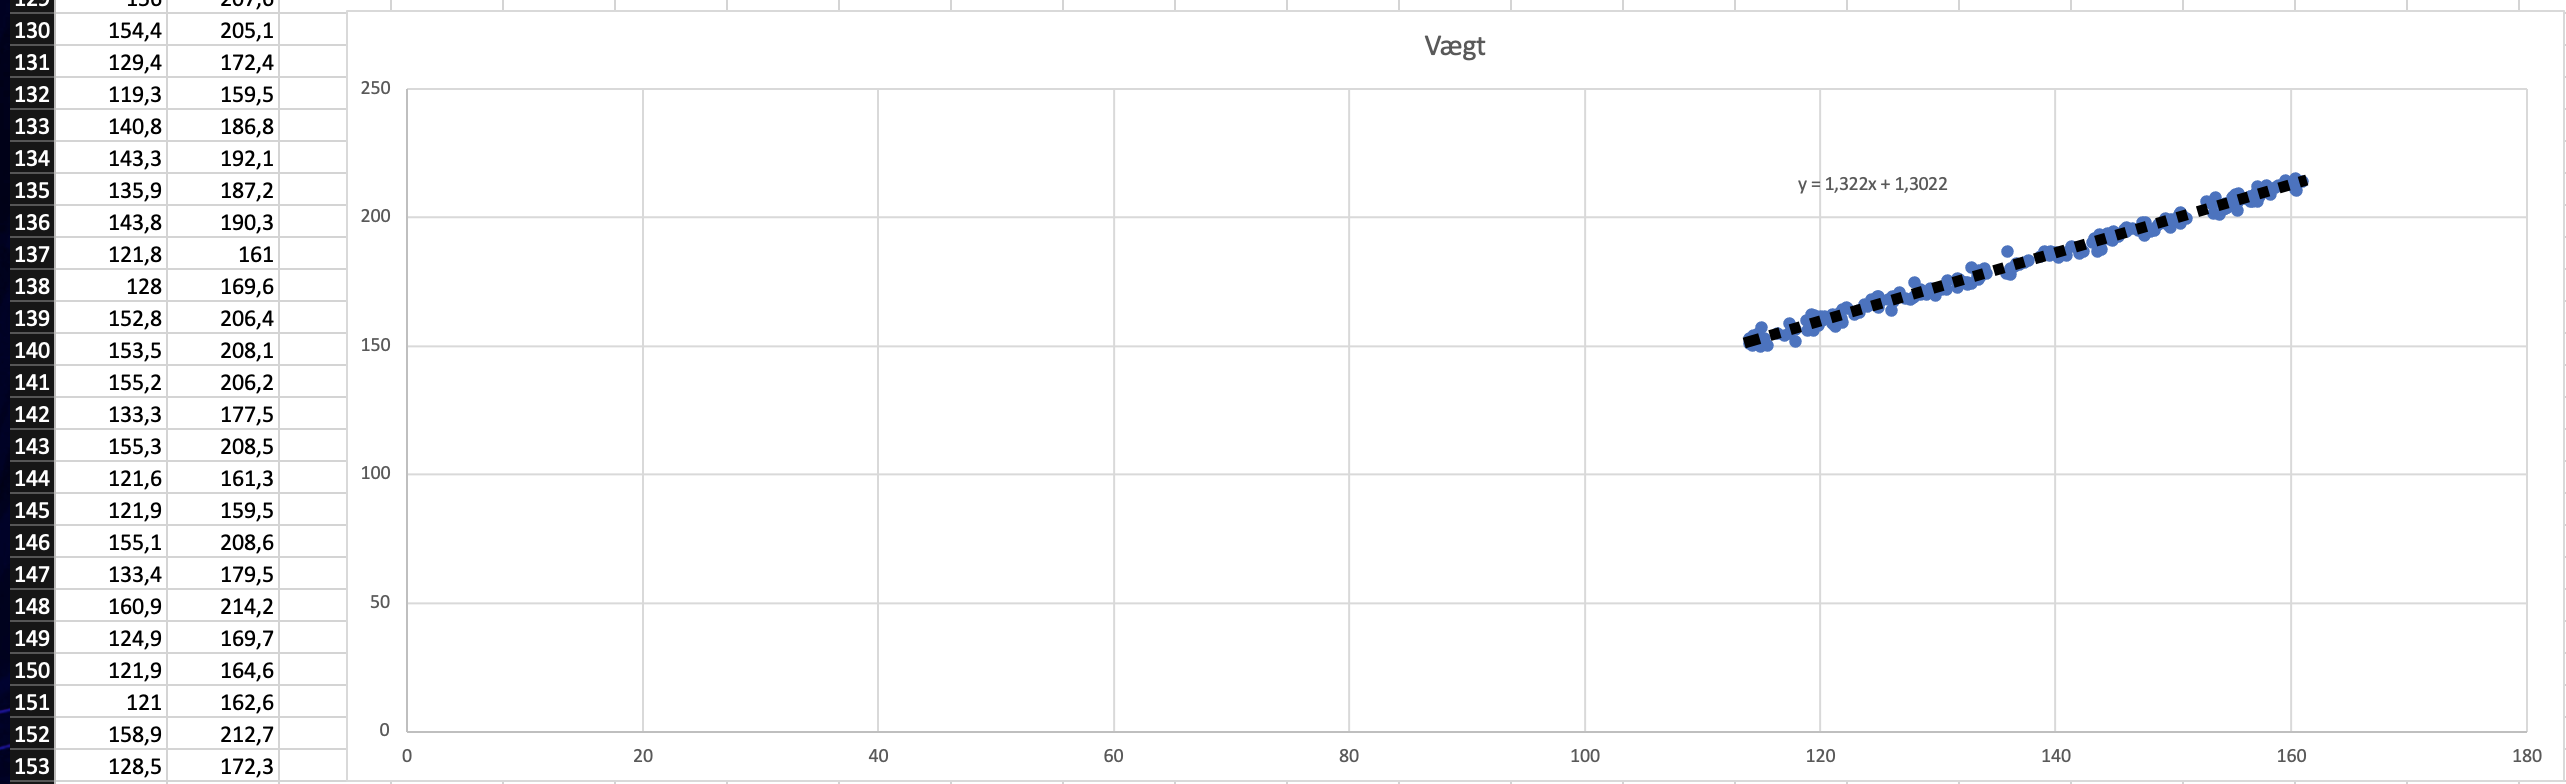
\includegraphics[width=\textwidth]{Excel.png }
\end{center}
\caption{Lineær regression lavet i Excel}
\label{fig:Excel}
\end{figure}

\begin{question}{Opgave 12 - Model for bro}{}
  Dronning Alexandrines Bro består af en række buer fastgjort på bropiller og en kørebane.
I en model i et koordinatsystem med enheden meter på begge akser kan den del af den midterste bue, der ligger over bropillerne, beskrives ved den positive del af grafen for 
\[
f(x)= -0,0104 \cdot x^2+ 41,7
\] 
I modellen er kørebanen vandret og ligger 26 meter over bropillerne.
\end{question}
Betegnelserne for bredde og længde illustreres i \cref{fig:bro}.
\begin{figure}[H]
\begin{center}
  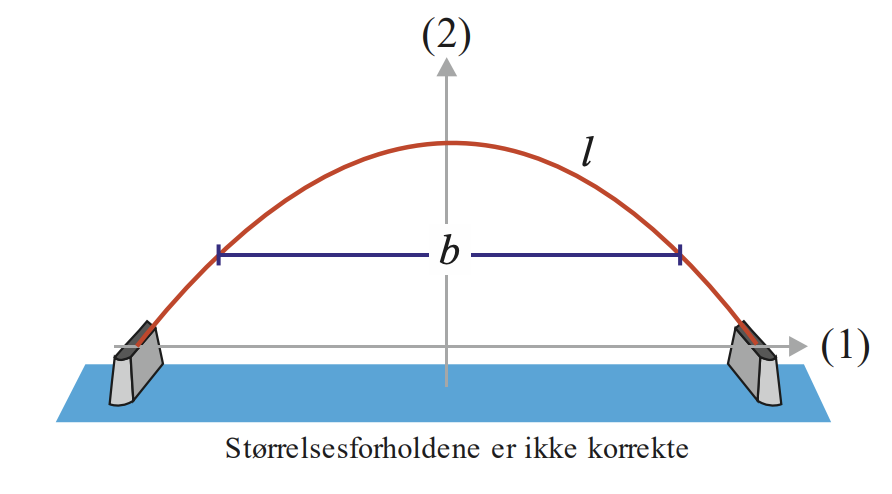
\includegraphics[scale=1]{bro.png}
\end{center}
\caption{Bredden $b$ og længden $l$ illustreret }
\label{fig:bro}
\end{figure}

\sol \\
\textbf{a.}
For at finde bredden $b$ af buen langs kørebanen, bestemmer vi først de to $x$-værdier, hvor $f(x)= 26$.
\begin{equation*}
\begin{split}
  f(x)= 26 &\iff -0,0104 \cdot x^2 +41,7 =26\\
  &\iff 0,0104 \cdot x^2 = 15,7\\
  &\iff x=\sqrt{\frac{15,7}{0,0104}} \lor x=- \sqrt{\frac{15,7}{0,0104}} 
\end{split}
\end{equation*}
Bredden målt langs kørebanen må da være afstanden mellem disse.
\begin{equation*}
\begin{split}
  b&=\abs{\sqrt{\frac{15,7}{0,0104}} -\left(- \sqrt{\frac{15,7}{0,0104}} \right) } \\
  &=2 \cdot \sqrt{\frac{15,7}{0,0104}} \\
  &\approx 77,7
\end{split}
\end{equation*}
Bredden af buen målt langs kørebanen er altså $77,7 \;\unit{m} $.\\[1ex]
\textbf{b.}
For at bestemme længden $l$ af buen fra bropille til bropille, finder vi først de to $x$-værdier, hvor $f(x)= 0$. 
\begin{equation*}
\begin{split}
  f(x)= 0 &\iff -0,0104 \cdot x^2 +41,7 =0\\
  &\iff x=\pm \sqrt{\frac{41,7}{0,0104}} 
\end{split}
\end{equation*}
Vi kan nu bestemme kurvelængden af grafen for $f$ mellem de to bropiller, hvilket gøres med CAS (se \cref{fig:buelængde}).
\begin{equation*}
\begin{split}
  l&=\int_{-\sqrt{\frac{41,7}{0,0104}} }^{\sqrt{\frac{41,7}{0,0104}} } \sqrt{1+f'(x)^2}  \,dx\\
  &=\int_{-\sqrt{\frac{41,7}{0,0104}} }^{\sqrt{\frac{41,7}{0,0104}} } \sqrt{1+\left(-0,0208x\right) ^2}  \,dx\\
  &\approx 157,06
\end{split}
\end{equation*}
Altså er længden af buen fra bropille til bropille $157,06 \;\unit{m} $ ifølge modellen. 
\begin{figure}[H]
\begin{center}
  \includegraphics[width=\textwidth]{buelængde.png}
\end{center}
\caption{Kurvelængden udregnet med CAS}
\label{fig:buelængde}
\end{figure}

\begin{question}{Opgave 13 - Bygningstag og funktion af to variable}{}
  I en model kan taget af en bygning beskrives ved grafen for funktionen
$$f(x,y)=0,88\cdot y\cdot\sin(0,63x)+2,2,\quad-7,5\leq x\leq7,5\text{og}-2,5\leq y\leq2,5,$$
hvor $f(x,y)$ beskriver tagets højde over broen (målt i meter).
I modellen er broen placeret i $xy$-planen.
\end{question}
\sol \\
\textbf{a.}
For at bestemme tagets højde over broen ved $x=0$ og $y=0$, beregner vi funktionens værdi $f(0,0)$. 
\begin{equation*}
\begin{split}
  f(0,0)&= 0,88 \cdot 0 \cdot \sin\left(0,63 \cdot 0\right) +2,2 \\
  &=2,2
\end{split}
\end{equation*}
Når $x=0$ og $y=0$ er tagets højde over broen altså $2,2 \;\unit{m} $. \\[1ex]
\textbf{b.} 
Grafen for $f$ tegnes i GeoGebra, og ses i \cref{fig:tag}. 
\begin{figure}[H]
\begin{center}
  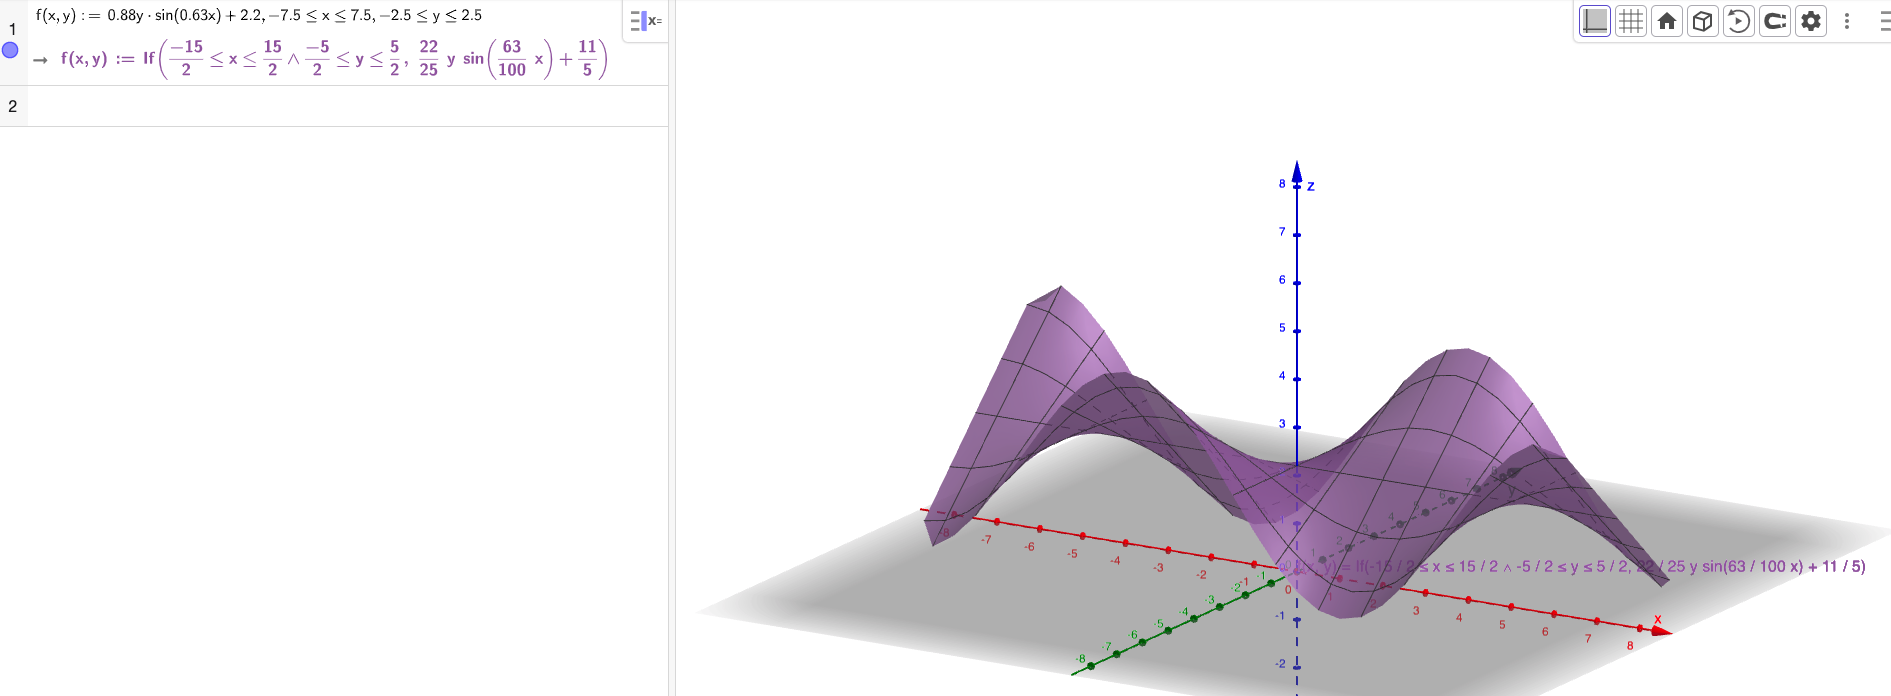
\includegraphics[width=\textwidth]{tag.png}
\end{center}
\caption{Grafen for $f$ tegnet i GeoGebra}
\label{fig:tag}
\end{figure}
\noindent Det oplyses, at afgrænsningen af taget mod syd kan beskrives ved snitkurven givet ved $g(x) =f(x,2.5)$. \\[1ex]
\textbf{c.}
For at bestemme tagets maksimale højde over broen mod syd, bestemmer vi først et udtryk for $g(x)$ udtrykt ved $x$. 
\begin{equation*}
\begin{split}
  g(x)&= f(x,2.5)\\
  &=0,88 \cdot 2,5 \cdot \sin\left(0,63x\right) +2,2\\
  &=2,2 \cdot \sin\left(0,63x\right) +2,2
\end{split}
\end{equation*}
Der må gælde, at $Dm(g)=[-7,5;7,5]$.
For at finde ekstremumssteder for $g$, løses ligningen $g'(x)=0$. 
\begin{equation*}
\begin{split}
  g'(x)=0 &\iff 2,2 \cdot 0,63 \cdot \cos\left(0,63x\right) =0\\
  &\iff \cos\left(0,63 x\right) =0\\
  &\implies  0,63 x = \frac{\pi }{2} \cdot \left(2k - 1\right), \quad k \in \mathbb{Z}\\
  &\iff x=\frac{50\pi }{63} \cdot \left(2k - 1\right), \quad k \in \mathbb{Z}
\end{split}
\end{equation*}
Når definitionsmængden for $g$ betragtes, ses det, at de eneste mulige løsninger må være 
\begin{equation*}
\begin{split}
  x=\frac{-50 \pi }{21} \lor x=\frac{-50 \pi }{63} \lor x=\frac{50 \pi }{63} \lor x=\frac{50 \pi }{21}
\end{split}
\end{equation*}
Fra grafen for $g$ i \cref{fig:ggraf}, er det dog tydeligt, at kun $x=\frac{-50 \pi }{21}$ og $x=\frac{50 \pi }{63}$ er maksimumssteder. 
\begin{figure}[H]
\begin{center}
  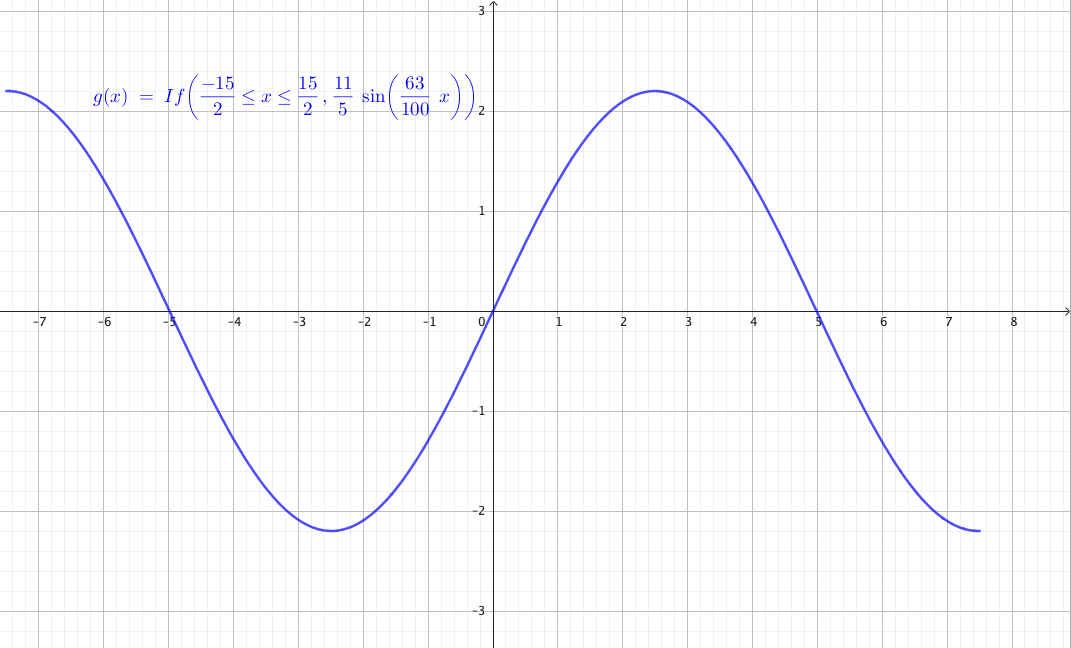
\includegraphics[width=\textwidth]{ggraf.png}
\end{center}
\caption{Grafen for $g$ tegnet i GeoGebra }
\label{fig:ggraf}
\end{figure}
Vi bestemmer nu funktionens værdi ved de to maksimumssteder.
Da der for disse gælder, at $\cos\left(0,63 x\right) =0$, så må $\sin\left(0,63 x\right) =1$, og vi har da
\begin{equation*}
\begin{split}
  g\left(\frac{-50 \pi }{21}\right) &= g\left(\frac{50 \pi }{63}\right)\\
  &=2,2 \cdot 1 +2,2\\
  &=4,4
\end{split}
\end{equation*}
Altså er tagets maksimale højde over broen mod syd $4,4 \;\unit{m} $.
\begin{question}{Opgave 14 - Muserute og vektorfunktion}{}
  En mus kravler ud af sit musehul og går en tur langs en lukket rute. I en model kan ruten
beskrives ved parameterkurven for vektorfunktionen $\vec{s}$ givet ved

$$\vec{s}(t)=\begin{pmatrix}x(t)\\y(t)\end{pmatrix}=\begin{pmatrix}4\cdot t-t^2\\t^3-9\cdot\mathfrak{t}^2+20\cdot t\end{pmatrix},\:0\le t\le4,$$

hvor $(x(t),y(t))$ betegner musens position til tidspunktet $t$ (målt i minutter) i et
koordinatsystem med enheden meter på begge akser. Musehullet er placeret i punktet
(0,0).
\end{question}
\sol \\
\textbf{a.}
Parameterkurven for vektorfunktionen $\va{s} $ tegnes i GeoGebra og ses i \cref{fig:rute}. 
\begin{figure}[H]
\begin{center}
  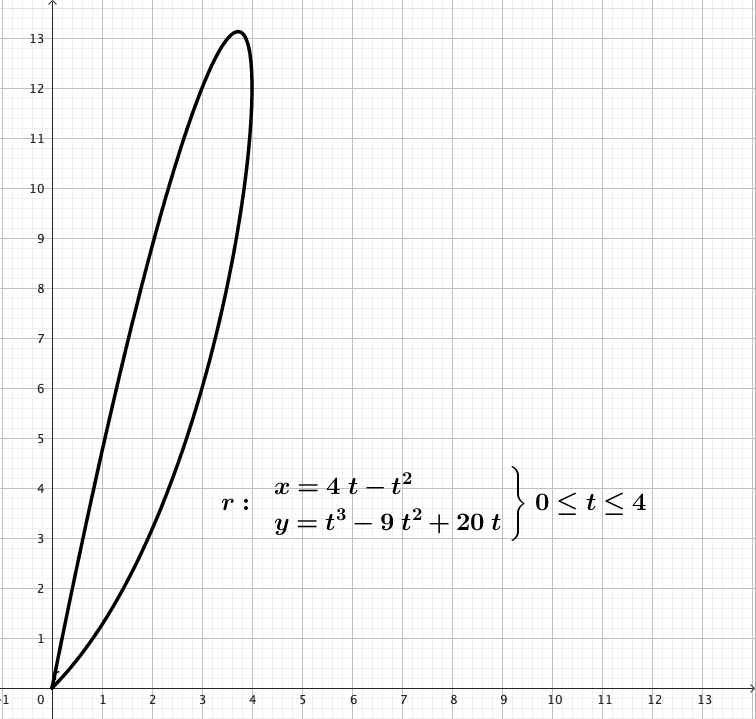
\includegraphics[width=0.7\textwidth]{rute.png}
\end{center}
\caption{Parameterkurve for $\va{s} $ tegnet i GeoGebra }
\label{fig:rute}
\end{figure}
\noindent \textbf{b.}
For at bestemme $\abs{\va{s}'(1)} $ finder vi først et udtryk for den afledede funktion for $s$. 
\begin{equation*}
\begin{split}
  \va{s}'(t)&=\mqty(\dv{t} \left(4t-t^2\right) \\ \dv{t} \left(t^3-9t^2+20t\right) ) \\
  &=\mqty(-2t+4\\ 3t^2-18t+20) 
\end{split}
\end{equation*}
Vi kan nu beregne $\abs{\va{s}'(1)} $.
\begin{equation*}
\begin{split}
  \abs{\va{s}'(1)} &=\abs{\mqty(-2 \cdot 1 + 4\\ 3 \cdot 1^2-18 \cdot 1 + 20) } \\
  &=\abs{\mqty(2\\ 5) } \\
  &=\sqrt{2^2+5^2} \\
  &=\sqrt{29} \\
  &\approx 5,39
\end{split}
\end{equation*}
Længden af den afledede funktion for stedvektoren $\va{s} $ må være musens fart. 
Altså har vi bestemt musens fart til tidspunktet $t=1$.
Musens fart efter 1 minut er altså $5,39 \;\unit{m/min} $.\\[1ex]
\textbf{c.}
For at bestemme tidspunktet, hvor musen er længst væk fra hullet, finder vi først et udtryk for musens afstand fra hullet.
Siden musehullet er i $(0,0)$, så må afstanden være længden af stedvektoren.
\begin{equation*}
\begin{split}
  \abs{\va{s} (t)} &=\abs{\mqty(4t-t^2\\ t^3-9t^2+20t) } \\
  &=\sqrt{\left(4t-t^2\right)^2+\left(t^3-9t^2+20t\right)^2} \\
  &=\sqrt{16t^2+t^4-8t^3+t^{6} - 18 \; t^{5} + 121 \; t^{4} - 360 \; t^{3} + 400 \; t^{2}}\\
  &=\sqrt{t^6-18t^5+122 t^4-368 t^3+416 t^2} 
\end{split}
\end{equation*}
For at finde ekstremumssteder, differentierer vi udtrykket med kædereglen, sætter lig nul og løser for $t$.
Bemærk, at afstanden ikke kan være $0$ her, da vi så vil have 0 i nævneren. 
\begin{equation*}
\begin{split}
  \dv{t} \sqrt{t^6-18t^5+122 t^4-368 t^3+416 t^2} =0 &\iff \frac{3t^5-45t^4+244t^3-552t^2+416t}{\sqrt{t^6-18t^5+122 t^4-368 t^3+416 t^2} }=0\\
  &\implies t \cdot \left(3t^4-45t^3+244t^2-552t +416\right) =0
\end{split}
\end{equation*}
Bemærk, at $t \neq 0$ her, da vi så dividerer med 0. 
Vi har da
\begin{equation*}
\begin{split}
  3t^4-45t^3+244t^2-552t +416=0 &\iff t \approx 1,504 \lor t=4
\end{split}
\end{equation*}
som løses med CAS (\cref{fig:CAS}).
Dog er $t \approx 1,504$ den eneste løsning, da $t \neq 4$ (for ellers divideres med 0).
Vi mangler nu blot at redegøre for, at $t \approx 1,504$ er et maksimumssted. 
Det fremgår tydeligt ved grafen for $\abs{\va{s} (t)} $, der ses i \cref{fig:mus}.
Altså er musen længst væk fra hullet efter $1,504$ minutter. 
\begin{figure}[H]
\begin{center}
  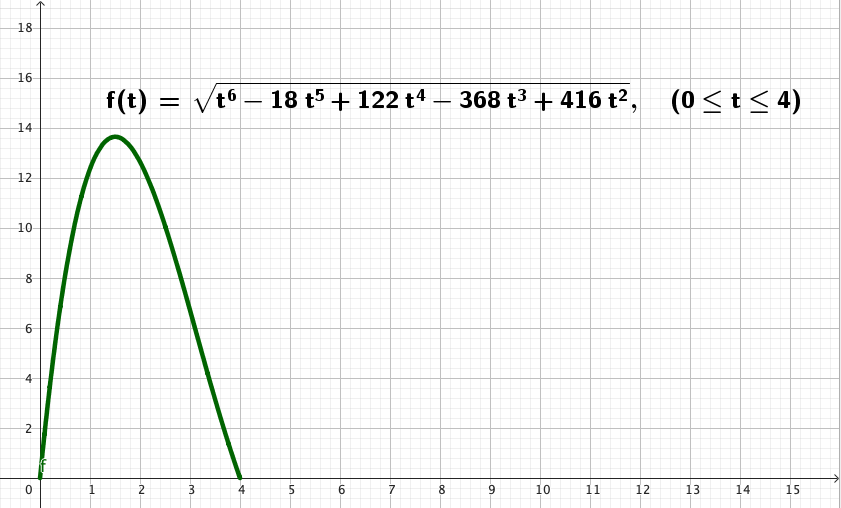
\includegraphics[width=\textwidth]{mus.png}
\end{center}
  \caption{Grafen for $\abs{\va{s} (t)} $}
\label{fig:mus}
\end{figure}


\begin{figure}[H]
\begin{center}
  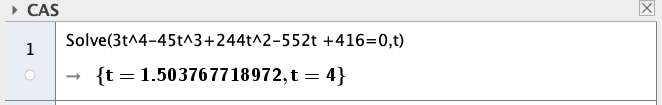
\includegraphics[width=\textwidth]{CAS.png}
\end{center}
\caption{Fjerdegradsligningen løst med CAS}
\label{fig:CAS}
\end{figure}


\end{document}
